\subsection{Datasets}
\par We studied 20 datasets, including 8 undirected graphs and 12 directed graphs. The details of the graphs are shown below.

\begin{table}[h]
\fontsize{8}{10}\selectfont
\begin{tabular}{llllll}
Dataset        & file                         & Category      & Directed & Sampled & Description                            \\ \hline
Skitter        & as-skitter.ungraph-75000.txt & Physical      & N        & Y       & autonomous systems on web              \\
Caida          & as-Caida.undir.txt           & Physical      & N        & N       & autonomous systems on web              \\
Enron          & email-Enron.ungraph.txt      & Communication & N        & N       & email records between employees        \\
EU institution & email-EuAll.txt              & Communication & Y        & N       & email records between employees        \\
Amazon         & com-amazon.ungraph-75000.txt & Co-occurence  & N        & Y       & bought X also bought Y                 \\
DBLP           & com-dblp.ungraph-75000.txt   & Coauthorship  & N        & Y       & coauthorship relationship              \\
Astro-ph       & ca-AstroPh.txt               & Coauthorship  & Y        & N       & coauthorship relationship              \\
Protein        & bio-protein-undir.txt        & Metabolic     & N        & N       & metabolic interaction between proteins \\
JDK            & soft-jdkdependency.txt       & Software      & Y        & N       & dependency between Java classes        \\
Spanish book   & text-spanishbook.txt         & Lexical       & Y        & N       & word following relationship            \\
Gnutella       & p2p-Gnutella31.txt           & Computer      & Y        & N       & connection between hosts               \\
Hep-Ph         & cit-HepPh.txt                & Citation      & Y        & N       & citation relationship                  \\
Hep-Th         & cit-HepTh.txt                & Citation      & Y        & N       & citation relationship                  \\
Cora           & cit-Cora.txt                 & Citation      & Y        & N       & citation relationship                  \\
Hamsterster    & soc-hamsterster.undir.txt    & Social        & N        & N       & social network friendship              \\
Youtube        & soc-Youtube-75000.undir.txt  & Social        & N        & Y       & social network friendship              \\
Slashdot       & soc-Slashdot0811-75000.txt   & Social        & Y        & Y       & directed friend/foe relationship       \\
Digg           & soc-digg.txt                 & Social        & Y        & N       & reply from one user to another         \\
Flickr         & soc-flickr-75000.txt         & Social        & Y        & Y       & directed friendship                    \\
Pokec          & soc-pokec-75000.txt          & Social        & Y        & Y       & directed friendship                    \\ \hline
\end{tabular}
\end{table}

In the following sections, we present our analysis on common features and distinctive patterns among these 20 dataset for various graph algorithms. Specifically, these algorithms include degree distributions, PageRank, weakly connected components, K-Core connected components with k=5, eigendecomposition and triangle count approximated from eigenvalues.

\subsection{Degree distributions}
\begin{figure}[H]
\begin{center}
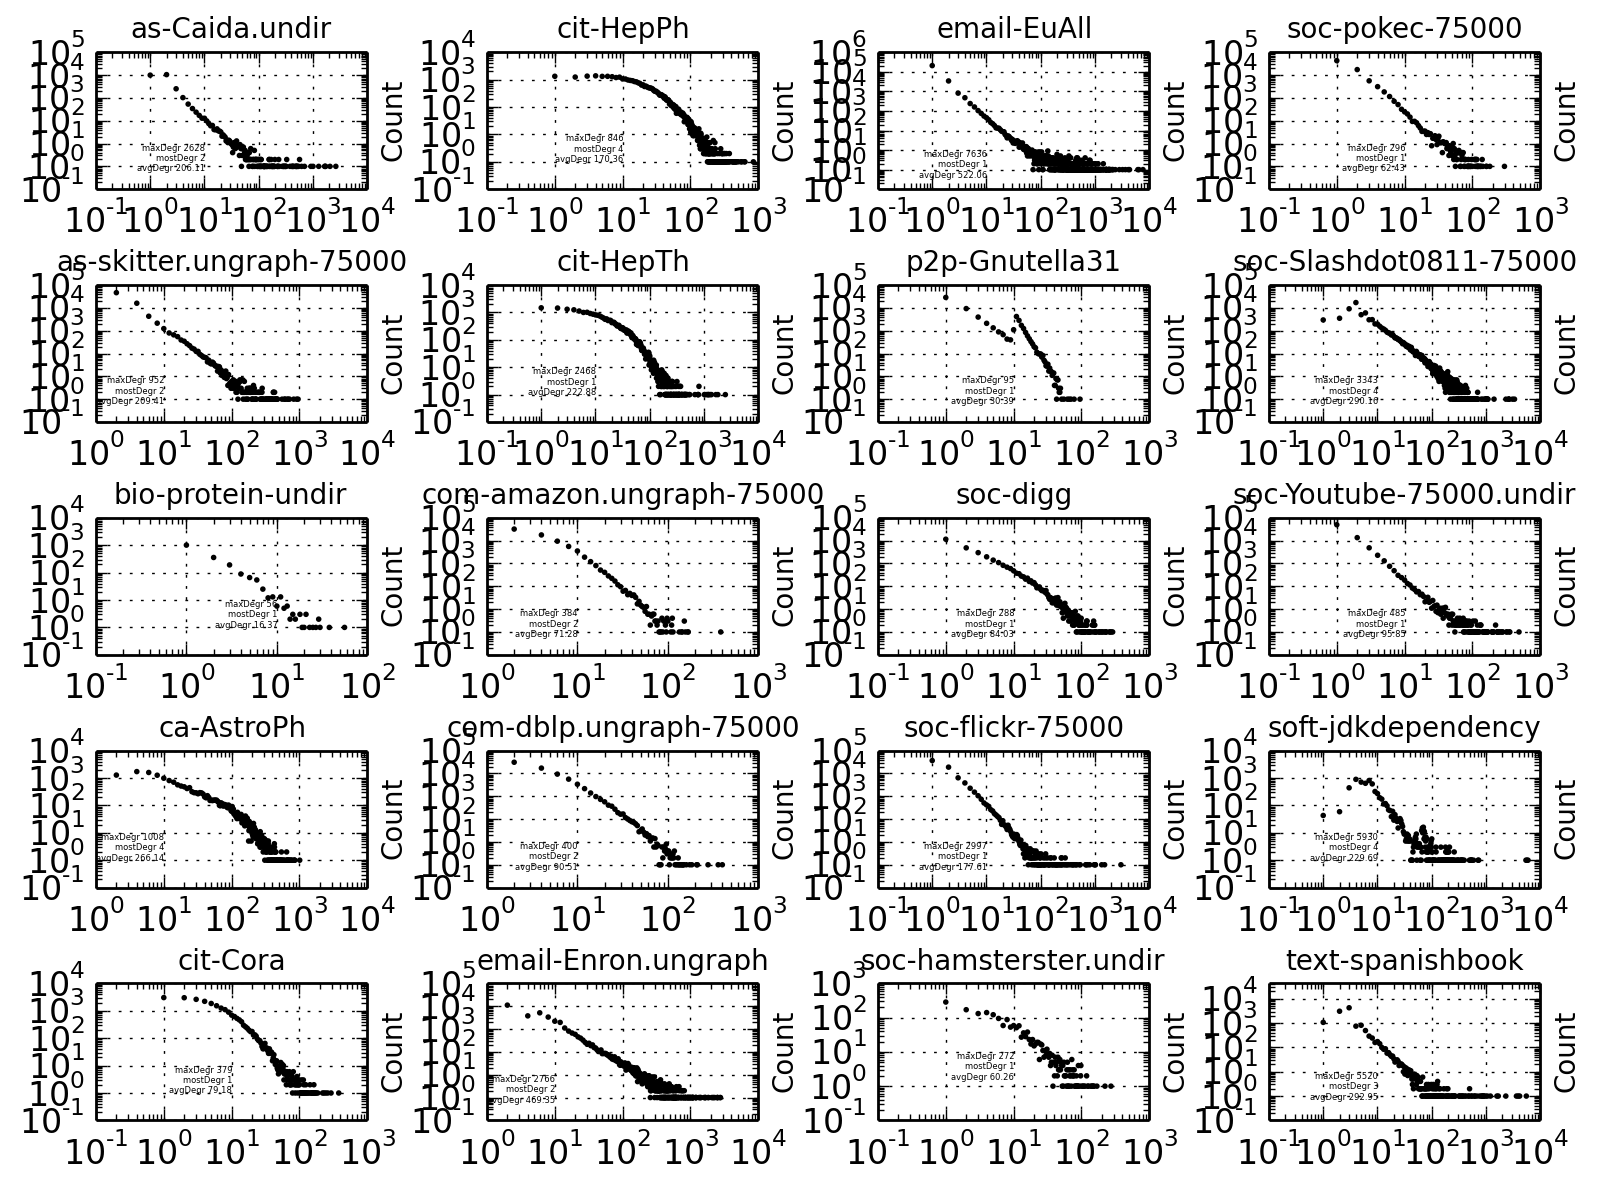
\includegraphics[width=\textwidth]{FIG/degreedist.png}
\caption{Degree distribution of 20 graphs}
\end{center}
\end{figure}

\par Degree distributions of most of the graphs follow the power law(see Figure 4 above). However, for some of the graphs, counts of the smallest 10 degrees exhibit different patterns from power law. These graphs are discussed below.

\begin{itemize}
\item \textbf{Hep-Ph} The degree which has most corresponding nodes is 4 instead of 1, implying that most publications in this section have more than one citation relationship with others. Counts of nodes with degree more than 4 follow the power law.
\item \textbf{Astro-Ph} The degree which has most corresponding nodes is 4 instead of 1, implying that most publications in this section have more than one citation relationship with others. Counts of nodes with degree more than 4 follow the power law.
\item \textbf{Gnutella} There is a radical increasing of degree count at degree around 10, implying that there may be a popular application that requires about 10 hosts to connect to each other in order to work.
\item \textbf{Slashdot} The degree which has most corresponding nodes is 4 instead of 1, implying that most users have 4 friend/foe relationship with others, which means the friend/foe marking functionality is popular among users. Count of nodes with degree more than 4 follows the power law.
\item \textbf{JDK} The degree which has most corresponding nodes is 4 instead of 1, implying that most classes have 4 dependency relationship with others. Also, the counts for nodes with degree 50 to 90 does not show a obvious decreasing trend but rather stable, indicating that complex dependency relationship between JDK classes is common. Another discovery is that there is one node with much higher degree than others.
\item \textbf{Spanish book} The degree which has most corresponding nodes is 3 instead of 1, implying that most words have 3 adjacency relationship with other words(including itself).
\end{itemize}

\par Also, we spot that Caida, Protein, Youtube, Hamsterster datasets all have nodes with zero degree, which is possibly because these datasets are produced by random walk sampling of original datasets, making some nodes isolated.

\begin{figure}[H]
\begin{center}
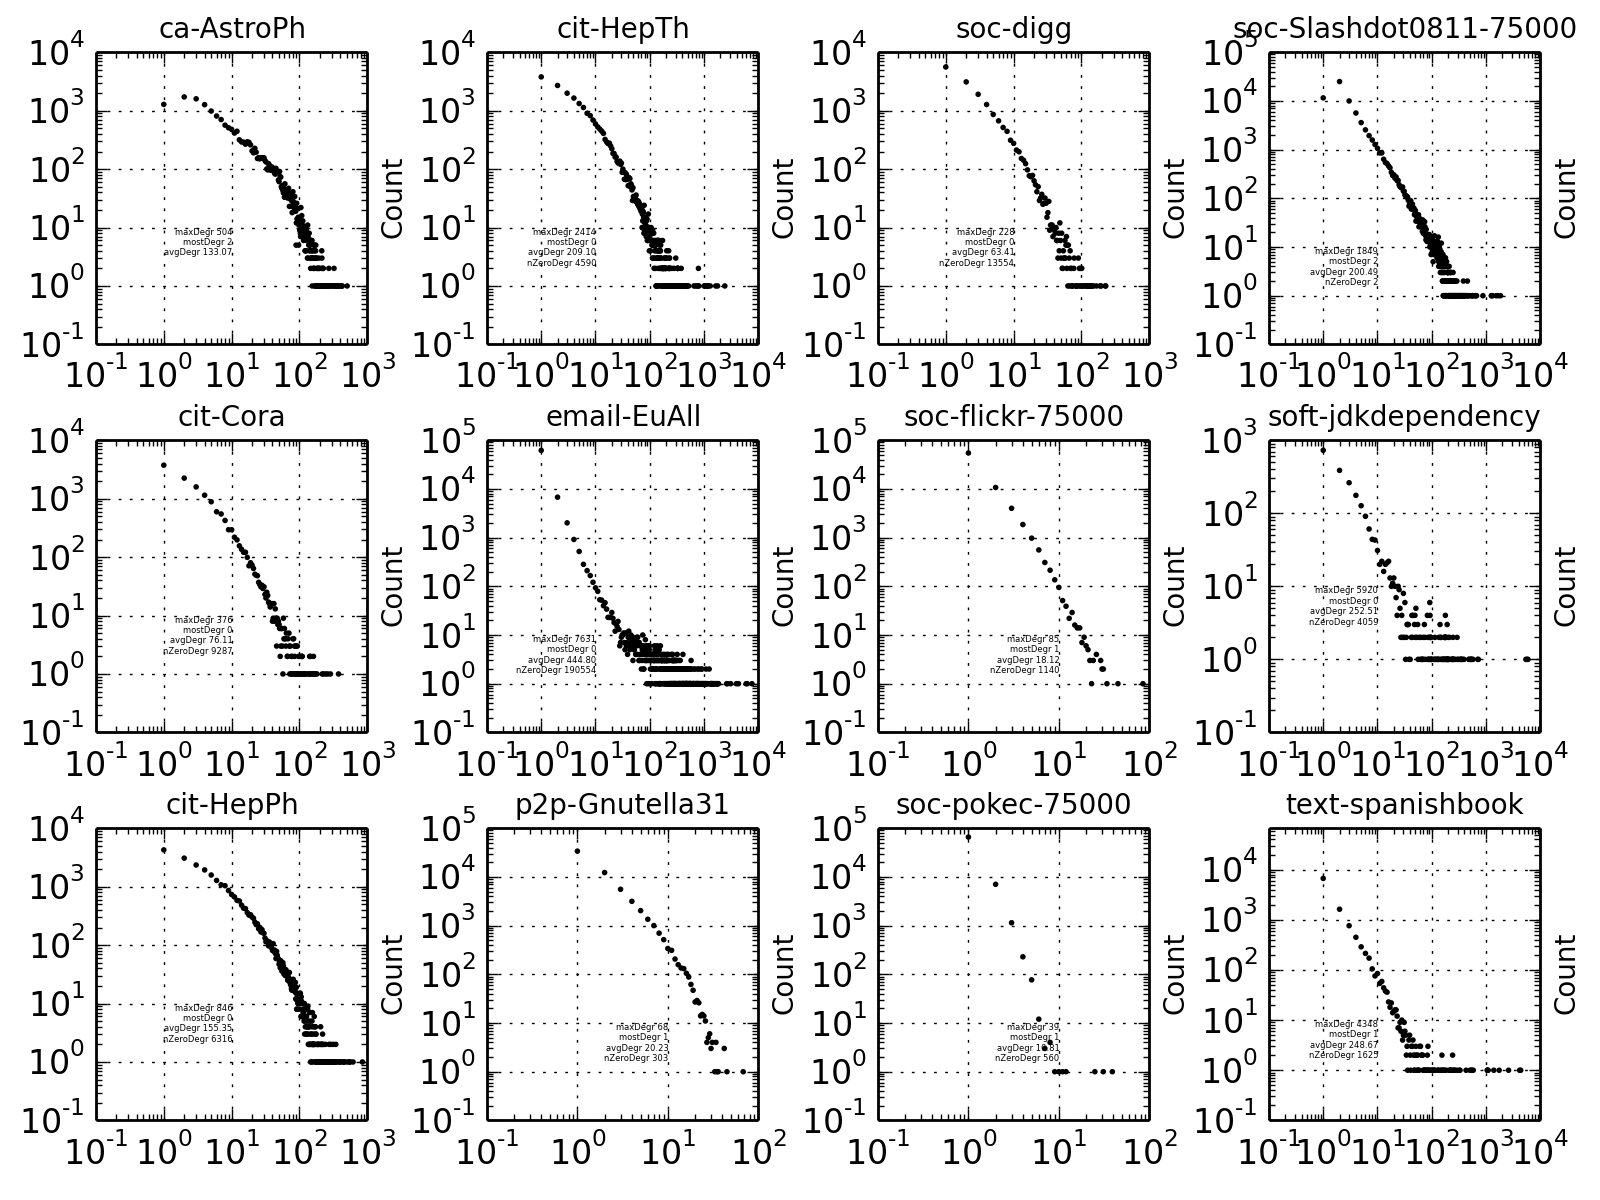
\includegraphics[width=\textwidth]{FIG/indegreedist.png}
\caption{Indegree distribution of 12 directed graphs}
\end{center}
\end{figure}

\par Indegree distributions of most of the directed graphs follow the power law(see Figure 5 above). But for 2 of the 12 directed graphs, not the whole indegree distribution obeys the power law. These graphs are discussed below.

\begin{itemize}
\item \textbf{Astro-Ph} The indegree which has most corresponding nodes is 2 instead of 1, indicating that most publications are cited by 2 publications.
\item \textbf{Slashdot} The indegree which has most corresponding nodes is 2 instead of 1, indicating that most users have received two friend/foe marking.
\end{itemize}

There are also some other interesting facts observed from the indegree distributions:
\begin{enumerate}
\item There are only two nodes with zero indegree in the \textbf{Slashdot} dataset, implying that almost all users have been marked as friend/foe by at least one user.
\item In \textbf{JDK} dataset, there is one node with much higher indegree than other nodes. This nodes most probably represents $java.lang.Object$ class. Also, most classes has zero indegree, indicating most classes are leaves in the class hierarchy, depended by no other classes.
\item In three citation graphs \textbf{Cora}, \textbf{Hep-Ph}, \textbf{Hep-Th}, most publications have zero indegree, indicating that most publications are not cited by others.
\end{enumerate}

\begin{figure}[H]
\begin{center}
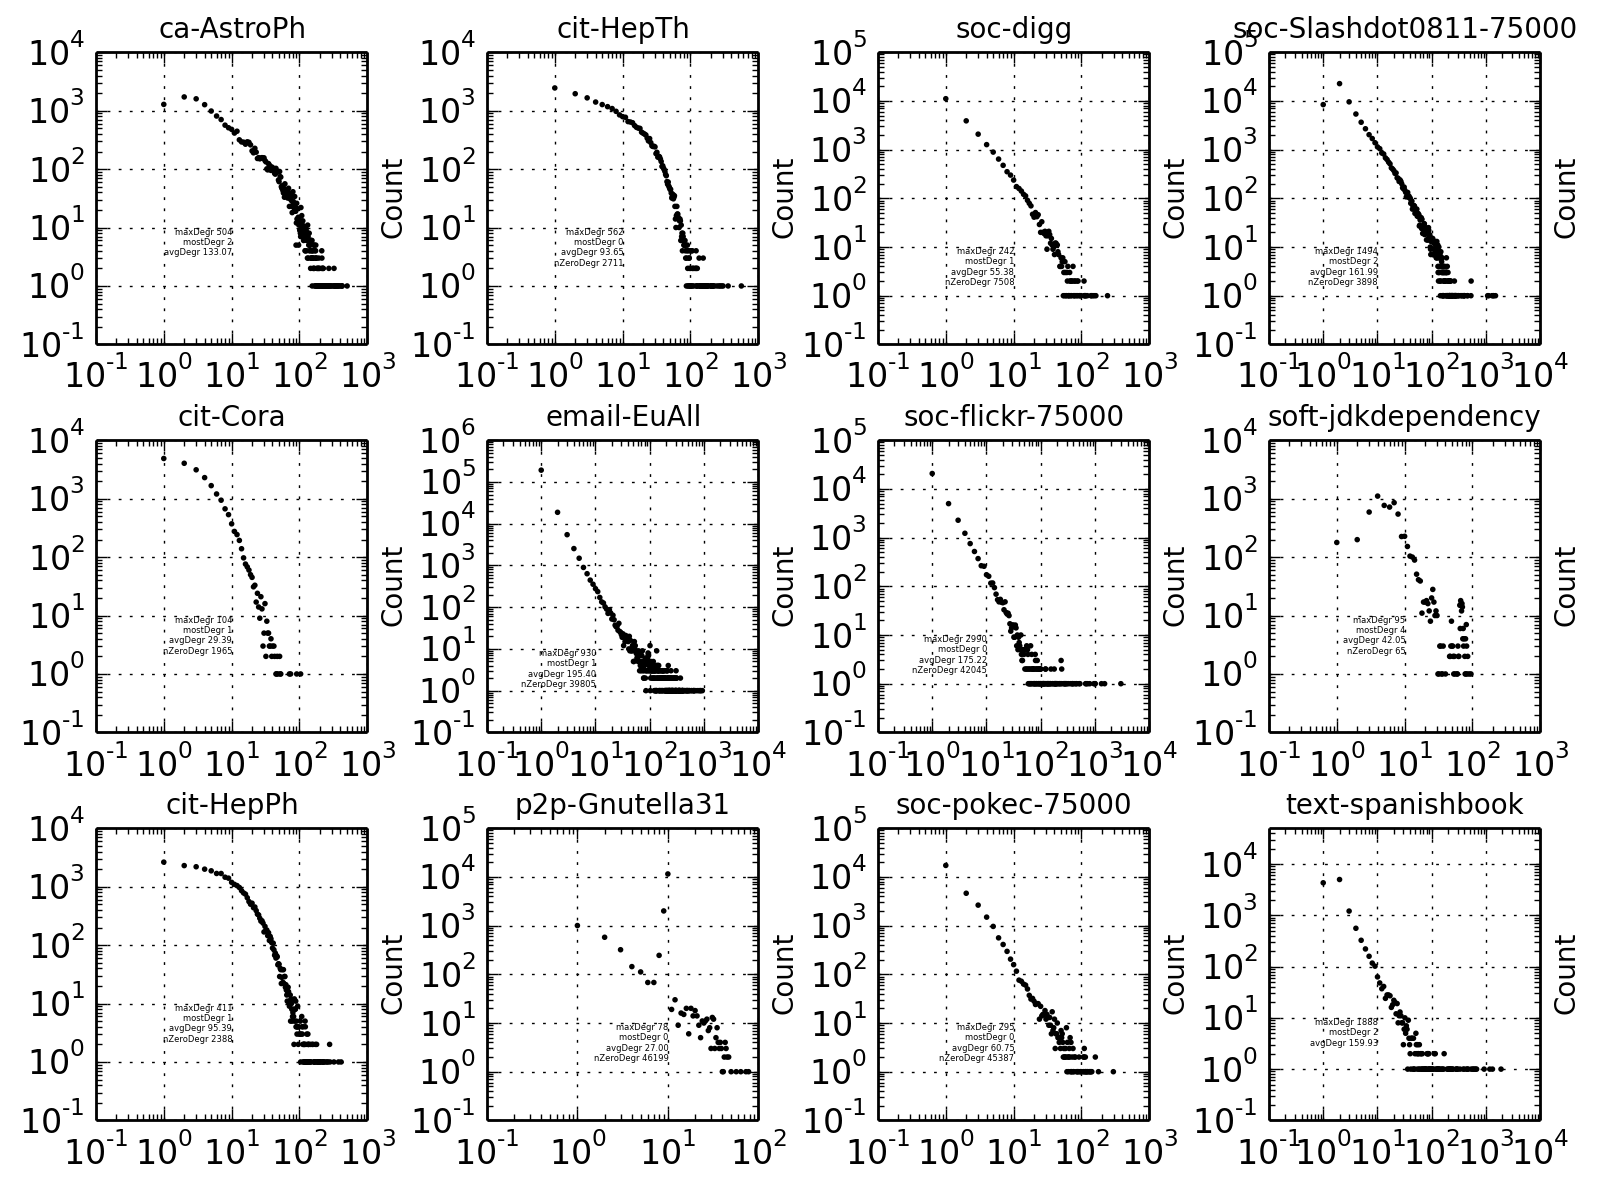
\includegraphics[width=\textwidth]{FIG/outdegreedist.png}
\caption{Outdegree distribution of 12 directed graphs}
\end{center}
\end{figure}

\par Outdegree distributions of most of the directed graphs follow the power law(see Figure 6 above). But for 5 of the 12 directed graphs, not the whole outdegree distribution obeys the power law. These graphs are discussed below.

\begin{itemize}
\item \textbf{Astro-Ph} The outdegree which has most corresponding nodes is 2 instead of 1, indicating that most publications cite 2 publications.
\item \textbf{Slashdot} The outdegree which has most corresponding nodes is 2 instead of 1, indicating that most users have made two friend/foe marking, again showing the popularity of this functionality.
\item \textbf{JDK} The outdegree which has most corresponding nodes is 4 instead of 1, indicating that most classes depend on 4 other classes. Also, only the middle part of the distribution, namely counts of nodes with outdegree 10 to 20, obey the power law.
\item \textbf{Gnutella} We spot a radical increasing of count starting from degree 7 to 10, and a radical decreasing from degree 10 to 11. This most probably indicates that the most common collaboration pattern in Gnutella network is for one host to connect to 8 to 10 hosts. Counts of nodes with degree more than 10 follow the power law.
\item \textbf{Spanish book} The outdegree which has most corresponding nodes is 2, indicating that most words in this book precedes two words(possibly itself). From the power law observed in the indegree and outdegree distribution of word adjacency in this book, it is clear that most words are used with only a few words together and few words are used very frequently with other words. This conforms to the nature of many languages.
\end{itemize}

Other interesting discoveries include:
\begin{enumerate}
\item In two of the social network datasets, \textbf{Flickr} and \textbf{Pokec}, nodes with zero outdegree is overwhelming, indicating that a substantial portion of users didn't actively make friends with other users, which means inactive users are quite common in social networks. In contrast, we spot in \textbf{Flickr} that one user has made about 2000 friends, more than twice of the second most, indicating that there is one extremely heavy user. Actually, there is a similar user in \textbf{Pokec} as well, but not so heavy. From these observations, we see that the activeness distribution caused by the nature of social network is the underlying reason of power law observed in both indegree and outdegree distribution.
\item Among three citation graphs, \textbf{Cora}, \textbf{Hep-Ph} and \textbf{Hep-Th}, most nodes in\textbf{Cora} has an outdegree of 1, much more than the nodes with zero outdegree, whereas in other two datasets the number of nodes with outdegree of 1 is close to the number of nodes with zero degree. This indicates that the research in Cora section is relatively more focused on established topics, while there are relatively more new topics in other two sections.
\end{enumerate}

\subsection{PageRank}
\begin{figure}[H]
\begin{center}
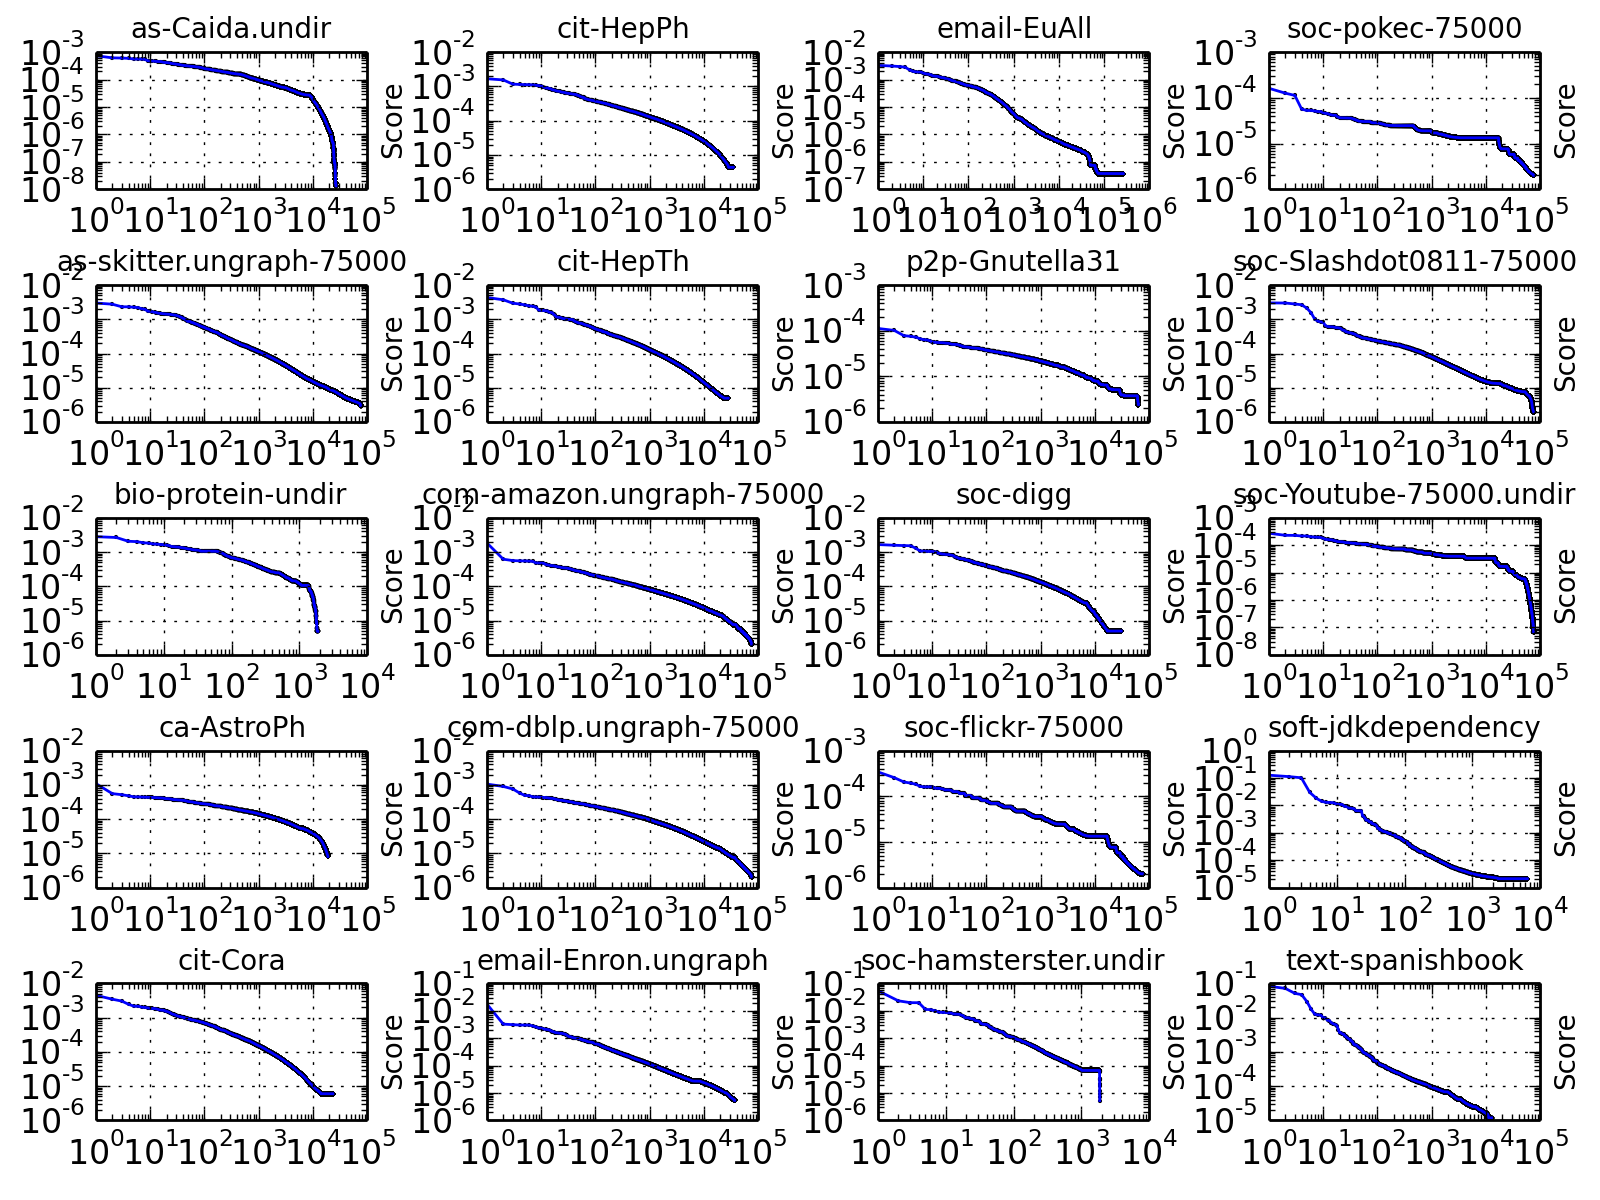
\includegraphics[width=\textwidth]{FIG/pagerank.png}
\caption{PageRank distribution of 20 graphs}
\end{center}
\end{figure}



\subsection{Weakly connected components}
\begin{figure}[H]
\begin{center}
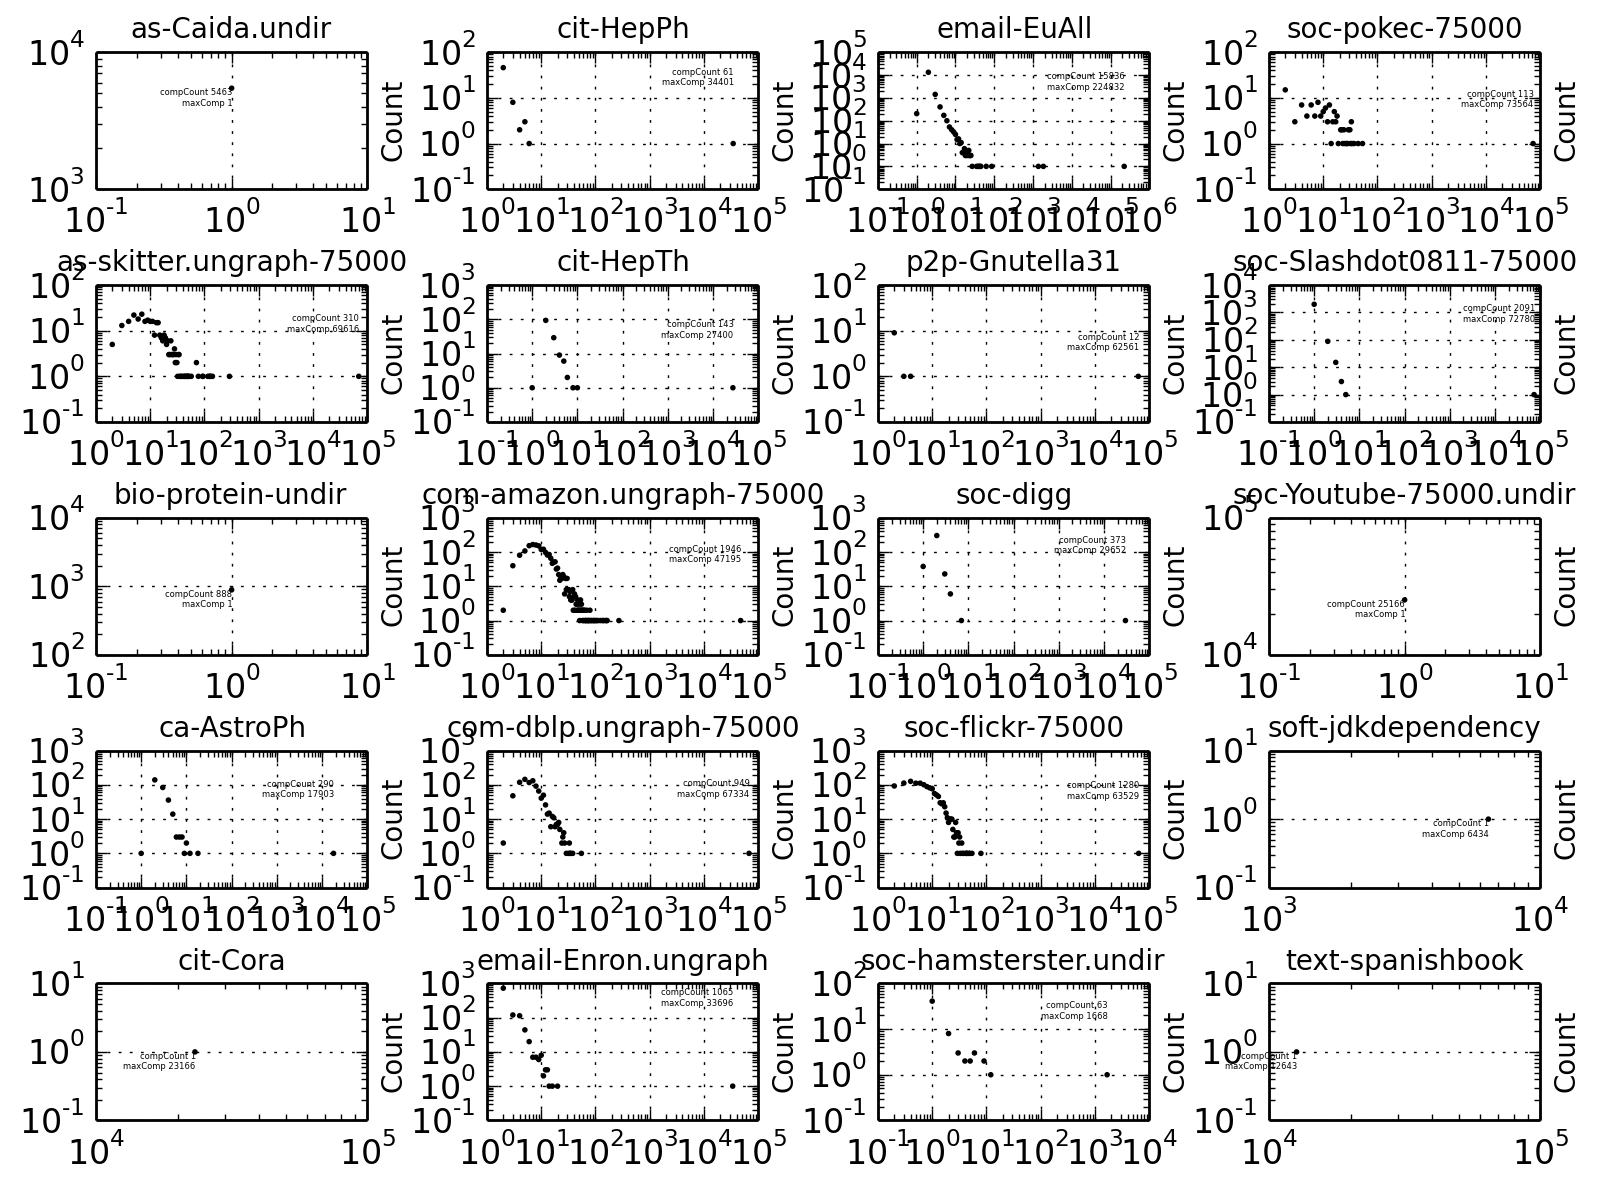
\includegraphics[width=\textwidth]{FIG/conncomp.png}
\caption{Weakly connected components distribution of 20 graphs}
\end{center}
\end{figure}

We plot the size of connected component and count of components with that size in Figure 8. From the figure we can see 5 datasets are fully connected. For the remaining datasets, all of them have a very large component relative to the sizes of the other components. Among these datasets, most of them exhibits a power relation in the count and component size for connected components with small sizes. But some graphs exhibit a different relationship, as discussed below.

\begin{itemize}
\item Some sampled datasets, such as \textbf{Skitter}, \textbf{Amazon}, \textbf{DBLP} and \textbf{Flickr}, count of the components with small components size increases with the component size, instead of decreasing.
\item \textbf{EU Institution} Count of components with only one node is far fewer than count of components with two nodes. One possible explanation of this distribution is that these nodes are spammers and since the spam emails they sent have been removed from the dataset, they are isolated from other nodes(users). As spammers are usually a small fraction of all the users, it explains why there is few components with only one node.
\item \textbf{Hep-Th, Astro-Ph} These two graphs share a common feature, there is only one component with only one node, far fewer than components of other small size. This is strange because these two graphs have no nodes with zero degree according to degree distribution. After checking the edge data, we found that these two graphs both have a node that have only one edge from it to itself. This can be explained in \textbf{Hep-Th} dataset since one publication can cite itself, however, for \textbf{Astro-Ph}, it may be an incorrect entry.
\item \textbf{Digg} Count of components with only one node is fewer than count of components with two nodes, indicating that few users haven't replied or received replies from other users. We can infer that most users in Digg tend to interact with other users.
\end{itemize}

\subsection{K-Core connected components with k=5}
\begin{figure}[H]
\begin{center}
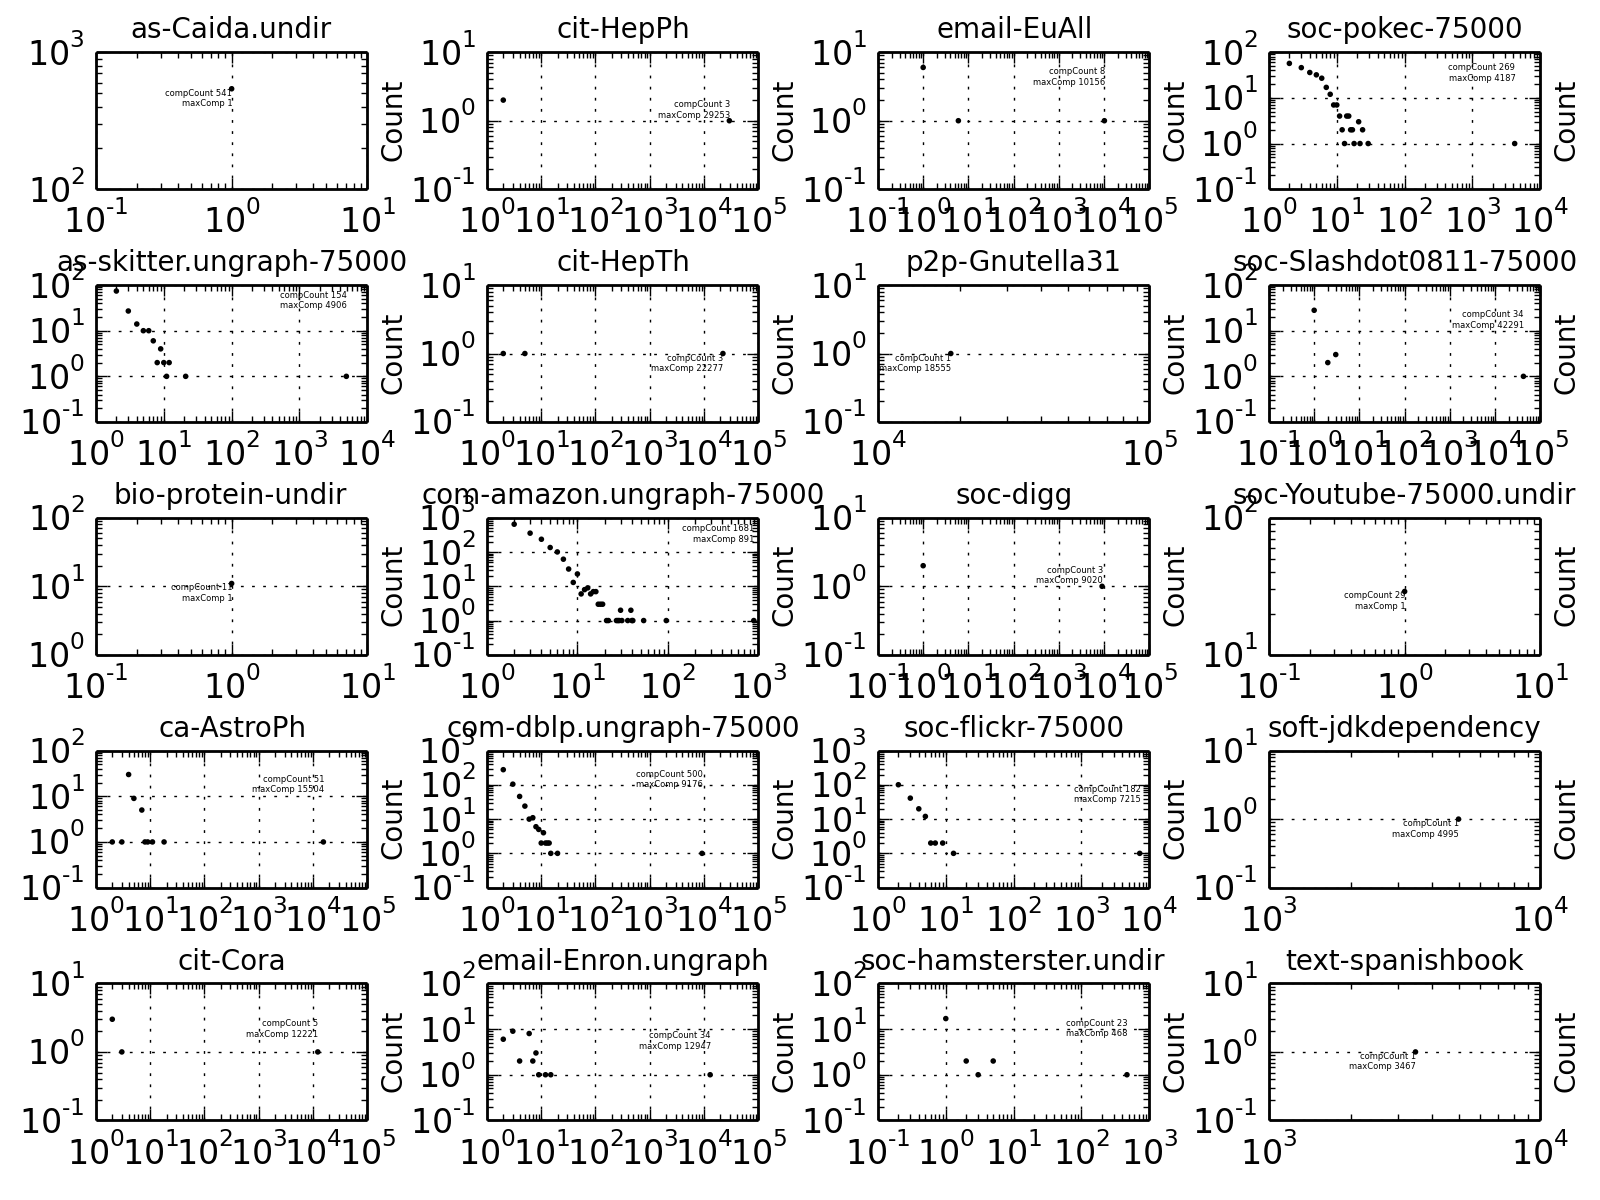
\includegraphics[width=\textwidth]{FIG/conncomp-kcore.png}
\caption{5-Core connected components distribution of 20 graphs}
\end{center}
\end{figure}

\subsection{Eigendecomposition}
\subsection{Triangle count}
\begin{figure}[H]
\begin{center}
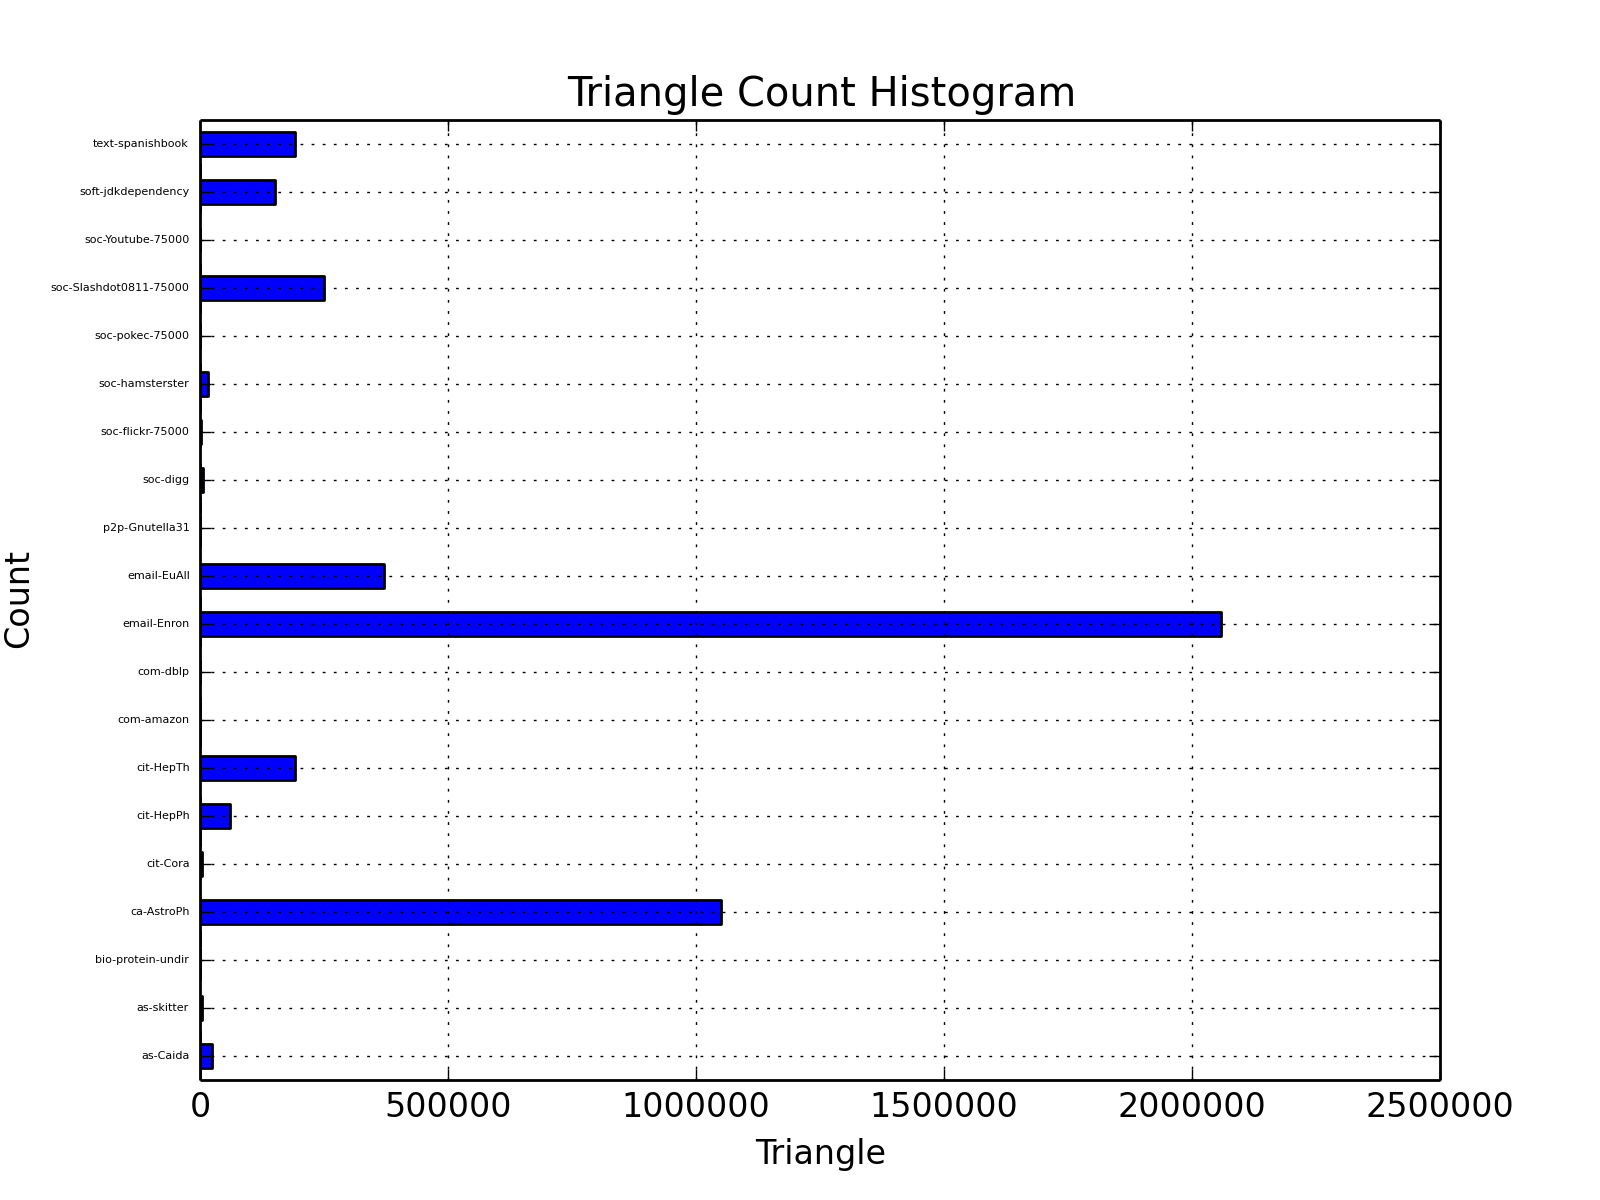
\includegraphics[width=\textwidth]{FIG/tria.png}
\caption{Count of triangle of 20 graphs, approximated from eigenvalues}
\end{center}
\end{figure}